\documentclass[sigconf]{acmart}

\begin{document}
%%
%% The "title" command has an optional parameter,
%% allowing the author to define a "short title" to be used in page headers.
\title{Poker Player Profiling: Heuristics vs. K-Means Clustering}

%%
%% The "author" command and its associated commands are used to define
%% the authors and their affiliations.
%% Of note is the shared affiliation of the first two authors, and the
%% "authornote" and "authornotemark" commands
%% used to denote shared contribution to the research.
\author{Lakshya Jain}
\email{lakshyajain@vt.edu}
\affiliation{%
  \institution{Virginia Tech}
}

\author{Aryan Shah}
\email{aryanmshah99@vt.edu}
\affiliation{%
  \institution{Virginia Tech}
}

\author{Shreya Aravindan}
\email{saravindan@vt.edu}
\affiliation{%
  \institution{Virginia Tech}
}

\author{Claire Shin}
\email{cshinh@vt.edu}
\affiliation{%
  \institution{Virginia Tech}
}

%%
%% The abstract is a short summary of the work to be presented in the
%% article.
\begin{abstract}
This paper compares rule-based heuristic profiling with K-means clustering for categorizing poker players by behavioral tendencies. We use the IRC Poker Database from the University of Alberta, extracting two features from player hand histories: Voluntarily Put Money in Pot (VPIP) and Pre-Flop Raise percentage (PFR). We filter the dataset for players with at least 30 hands and analyze a total of 16,439 players across three Texas Hold'em channels. Using the fixed VPIP and PFR heuristic baseline, players are assigned to four traditional archetypes: TAG, LAG, Fish, Rock. Conversely, the K-means approach groups players based on behavioral similarity in the feature space. Both methods are evaluated using silhouette scores. K-means at $K=4$ produces tighter and better-separated grouping than traditional heuristics by achieving a silhouette score of 0.4420, more than three times the heuristic baseline score of 0.1347. K-means also uncovers meaningful variation within the heuristic categories, particularly among more aggressive players. These results suggest that even a simple K-means approach can produce better clustering structures than the rule-based approach under silhouette-based evaluation.
\end{abstract}

%%
%% Keywords. The author(s) should pick words that accurately describe
%% the work being presented. Separate the keywords with commas.
\keywords{poker analytics, player profiling, clustering, K-means, heuristic labeling, unsupervised learning}

%%
%% This command processes the author and affiliation and title
%% information and builds the first part of the formatted document.
\maketitle

\section{Introduction}
Poker is a competitive decision-making game involving players betting money based on how advantageous their hand is and their judgment of opponents' cards and/or behavior. Understanding player behavior helps develop advantageous strategies by informing betting patterns, risk tolerance, and gameplay decisions.

In poker analysis, players are traditionally categorized into four different behavioral archetypes: Tight Aggressive (TAG), Loose Aggressive (LAG), Loose Passive (Fish), and Tight Passive (Rock). Players are grouped into different archetypes by two statistics: VPIP (Voluntarily Put Money in Pot) and PFR (Pre-Flop Raise percentage). These behavioral statistics measure player participation frequency and aggression levels.

In this study, we investigate whether unsupervised machine learning methods can provide meaningful behavioral player groupings from gameplay statistics. Specifically, we apply K-means clustering to player-level VPIP and PFR features and compare the resulting clusters against traditional heuristic-based poker classifications. This comparison allows us to evaluate how closely data-driven behavioral groupings align with the traditional categories.

\section{Related Work}
Poker player profiling has a long history in both the AI and poker analytics communities. Foundational techniques for opponent modeling in Texas Hold'em were introduced by Billings et al.~\cite{billings2002challenge}. Their work established VPIP and PFR as standard features for distinguishing player tendencies, demonstrating that aggregate behavioral statistics derived from hand histories can characterize players. In addition, Southey et al.~\cite{southey2005bayes} highlights the importance of pre-flop statistics as primary signals for player classification. 

Clustering methods have also been widely applied beyond poker-specific research. Drachen et al.~\cite{drachen2012guns} applied K-means clustering to player telemetry data in a commercial video game. The results showed that unsupervised methods can recover interpretable behavioral archetypes without any pre-defined labels. These findings parallel our own, as the K-means approach split the heuristic LAG category into meaningfully distinct subgroups, suggesting that data-driven clusters can often reveal substructures invisible to the heuristic approach. Another approach, by Bauckhage et al.~\cite{bauckhage2012players}, emphasizes that clustering player activity patterns can be used to identify behavioral transitions over time. 

Hartigan and Wong~\cite{hartigan1979kmeans} remains the standard K-means algorithm used in this study. We measure cluster quality using the silhouette coefficient, which measures the ratio of intra-cluster cohesion to inter-cluster separation, introduced by Rousseeuw~\cite{rousseeuw1987silhouettes}. We use the silhouette score as an appropriate method of evaluating the unsupervised K-means approach against a heuristic baseline as it does not require ground-truth labels. 

Though the traditional heuristic baseline is commonly used in applied poker analytics to assign players to archetypes such as TAG, LAG, Fish, and Rock~\cite{billings2002challenge}, the threshold-based classifiers are sensitive to cutoff values if they are not adapted to the underlying data distribution ~\cite{fernandez2016generic}. This limitation motivates our study on whether an unsupervised method can better group players than a fixed-threshold heuristic on the same feature space.

\section{Methodology}
This section describes the dataset, pre-processing pipeline, feature engineering process, heuristic profiling framework, and K-means clustering methodology used for behavioral player analysis.

\subsection{Dataset}
We use the IRC Poker Database provided by the University of Alberta~\cite{irc_poker_dataset}, which contains millions of Texas Hold’em poker hands collected from Internet Relay Chat (IRC) servers. The dataset is well suited for behavioral analysis as it provides gameplay records that capture player participation and betting behavior over the long term and across many hands. 

The raw dataset consists of hand history logs, where each entry corresponds to a single poker hand. Each record contains information such as a unique hand identifier, the number of participating players, aggregated betting activity across multiple betting rounds (pre-flop, flop, turn, and river), and the list of players involved in the hand. In poker analytics, hand histories provide a detailed record of gameplay actions and are commonly used to calculate behavioral statistics. 

An example of the dataset structure is shown in Table~\ref{tab:dataset_sample}. Entries such as ``2/50'' represent the number of bets and the corresponding pot size during a particular stage of play. Since the dataset does not directly provide player-level statistics, pre-processing was required to obtain the hand histories and aggregate player actions across many hands. 

As the games in this dataset were played between 1995 and 2001, any patterns that we identify might not reflect how modern poker is played. Given the size of the original dataset, we also used sampled subsets during pre-processing and exploratory analysis to keep the work manageable while still retaining representative player behavior. 

\begin{table}[t]
\centering
\small
\caption{Sample Entries from the IRC Poker Dataset}
\label{tab:dataset_sample}
\begin{tabular}{c c c c c c}
\toprule
Hand ID & \#Players & Pre-Flop & Flop & Turn & River \\
\midrule
797223441 & 3 & 2/20 & 2/40 & 0/0 & 0/0 \\
797223474 & 6 & 2/50 & 2/70 & 2/110 & 2/190 \\
797223636 & 7 & 4/80 & 4/120 & 2/160 & 2/200 \\
797223883 & 7 & 5/50 & 5/50 & 4/130 & 2/170 \\
\bottomrule
\end{tabular}
\end{table}

\begin{table}[t]
  \caption{Dataset Summary}
  \label{tab:dataset-summary}
  \centering
  \begin{tabular}{lr}
    \toprule
    Statistic & Value \\
    \midrule
    Total Parsed Hand Records & 19,580,075 \\
    Channel-Level Unique Player Sum & 30,559 \\
    Retained Players ($\geq$ 30 hands) & 16,439 \\
    Clustering Features & 2 \\
    \bottomrule
  \end{tabular}
\end{table}

\subsection{Pre-processing}
The pre-processing pipeline parsed player actions from numerous hand histories and calculated the aggregate statistics across all the observed hands. During preprocessing, noise and inactive participants (i.e., participants with fewer than 30 hand samples) were removed from the dataset. This process ensured meaningful player representations for analyzing long-term behavioral tendencies. 

From the aggregated gameplay data, VPIP and PFR were calculated. VPIP measures how frequently a player voluntarily enters pots, while PFR measures how often a player raises before the flop. Together, these metrics capture player looseness and aggression. 

Additional pre-processing steps included:

\begin{itemize}
    \item Aggregating hand-level actions into player-level summaries,
    \item Normalizing percentage-based behavioral metrics,
    \item Computing total hands played for reliability analysis.
\end{itemize}

Figure~\ref{fig:vpip-pfr-distributions} shows the resulting feature distributions after pre-processing. The VPIP distribution shows a wide spread centered around moderately loose play. On the other hand, the PFR distribution is strongly right-skewed. This indicates that passive pre-flop behavior, indicated by the low PFR, is comparatively more common, while aggressive pre-flop raising behavior is less common. After observing this skewed participation patterns during pre-processing, we used a minimum hand-count filter before clustering. 

\begin{figure}[t]
  \centering
  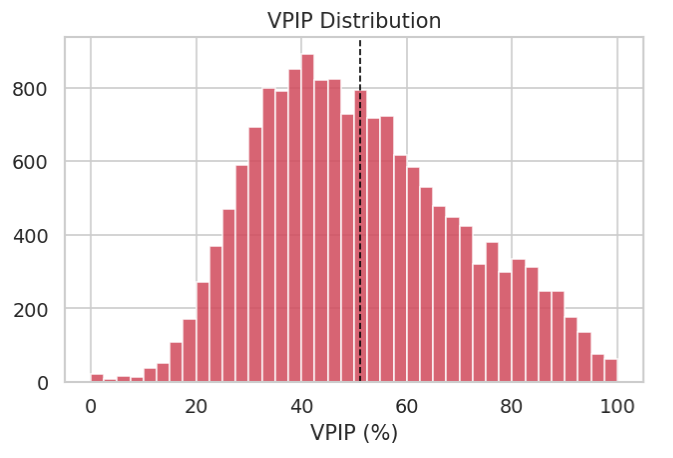
\includegraphics[width=\linewidth]{figures/vpip_distribution.png}
  \vspace{0.5em}
  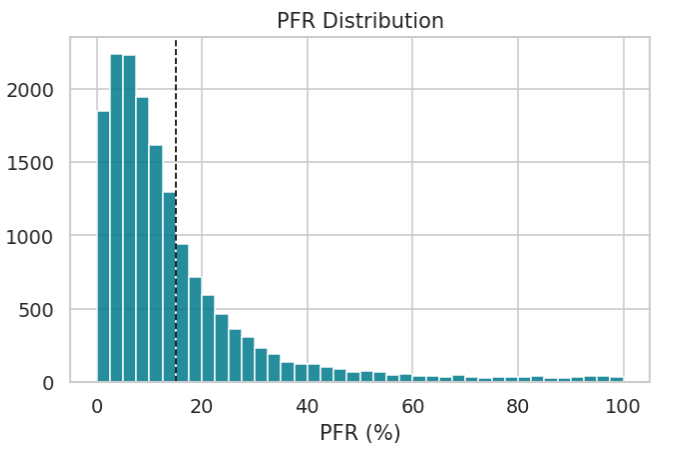
\includegraphics[width=\linewidth]{figures/pfr_distribution.png}
  \caption{Distributions of VPIP and PFR after pre-processing and player-level aggregation. VPIP exhibits a broader spread centered around moderately loose play, while PFR is strongly right-skewed, indicating that highly aggressive pre-flop raising behavior is comparatively uncommon.}
  \label{fig:vpip-pfr-distributions}
\end{figure}

\subsection{Feature Engineering}
Player-level behavioral features were engineered from the parsed hand histories to capture long-term poker playing tendencies. The pre-processing pipeline aggregated hand-level statistics for each player and computed summary metrics describing participation frequency and pre-flop aggression.

In addition to VPIP and PFR, many participation-related statistics were computed. These include total hands played, total channels played, and number of active months observed. These statistics were used for filtering, validation, and reliability analysis rather than direct clustering. The final clustering analysis used VPIP and PFR for heuristic profiling and K-means clustering. 

\begin{table}[t]
  \caption{Engineered Player-Level Features}
  \label{tab:features}
  \centering
  \begin{tabular}{lp{0.55\linewidth}}
    \toprule
    Feature & Description \\
    \midrule
    VPIP & Percentage of hands where a player voluntarily invested chips pre-flop. \\
    PFR & Percentage of hands where a player raised before the flop. \\
    Total Hands & Total number of parsed hands associated with a player. \\
    Channels Played Count & Number of poker channels in which the player appeared. \\
    Months Played Count & Number of months during which the player was active. \\
    \bottomrule
  \end{tabular}
\end{table}

\subsection{Heuristic Player Profiling}
A rule-based heuristic profiling system was developed to categorize players into the four archetypes using their VPIP and PFR values, as traditionally done in poker. 

VPIP was used to distinguish between tight and loose players. Players with lower VPIP values participate in fewer hands and are therefore considered tighter, while players with higher VPIP values voluntarily enter more pots and are considered looser.

PFR was used to measure pre-flop aggression. Players with higher PFR values are considered more aggressive as they raise more frequently before the flop. Both VPIP and PFR jointly capture the participation frequency and pre-flop aggression. 

The heuristic labeling system used fixed threshold values of:
\begin{itemize}
    \item VPIP threshold: $25\%$
    \item PFR threshold: $15\%$
\end{itemize}

The resulting heuristic labels were used both for the exploratory analysis and for the comparison against the K-means clustering results.

\begin{table}[t]
  \caption{Heuristic Labeling Rules}
  \label{tab:heuristic-rules}
  \centering
  \begin{tabular}{lll}
    \toprule
    Profile & VPIP Condition & PFR Condition \\
    \midrule
    TAG (Tight Aggressive) & VPIP $< 25$ & PFR $\geq 15$ \\
    LAG (Loose Aggressive) & VPIP $\geq 25$ & PFR $\geq 15$ \\
    Rock (Tight Passive) & VPIP $< 25$ & PFR $< 15$ \\
    Fish (Loose Passive) & VPIP $\geq 25$ & PFR $< 15$ \\
    \bottomrule
  \end{tabular}
\end{table}

\subsection{K-Means Clustering}
K-means clustering used the two main behavioral features, VPIP and PFR, to identify player groupings directly from the poker data. The feature space was standardized prior to clustering to ensure that VPIP and PFR both contributed equally. 

Using the elbow method and silhouette analysis, the optimal number of clusters was evaluated. The elbow method examined the within-cluster sum of squared errors (inertia) across values of $K$, while silhouette scores measured the separation and cohesion quality of the resulting clusters.

Given these evaluation metrics, a four-cluster model was chosen as the most meaningful representation of the player population. The four-cluster choice also matched the number of archetypes used in the heuristic profiling.

To guarantee reproducibility and clustering stability, the K-means model was initialized with a fixed random seed and multiple initialization runs. The final clustering model assigned each player to one of four behavioral groups in the VPIP-PFR feature space.

After training, the centroid positions and average behavioral characteristics of each cluster were interpreted. Clusters with low VPIP and PFR values corresponded with tighter more passive players. Clusters with high VPIP and PFR values corresponded with looser and more aggressive players. The intermediate clusters captured players with average aggression and participation. 

\begin{figure}[t]
  \centering
  
\includegraphics[width=\linewidth]{figures/holdem_kmeans_model_selection.png}
  \caption{Model selection results for K-means clustering. The elbow method evaluates within-cluster inertia across candidate values of $K$, while silhouette analysis measures cluster separation quality.}
  \Description{Plots showing inertia and silhouette scores for different K-means cluster counts used to determine the optimal number of clusters.}
  \label{fig:elbow-plot}
\end{figure}

\section{Results and Evaluation}
This section presents the exploratory analysis, heuristic profiling outcomes, clustering results, and quantitative evaluation comparing rule-based and unsupervised player segmentation approaches.

\subsection{Exploratory Data Analysis}
Exploratory data analysis (EDA) was first performed on a dataset of around 350 players. Once an overall understanding of the data was achieved, EDA was performed on a dataset containing 16,439 players. Table \ref{tab:eda-stats} summarizes the key statistics of the two clustering features.

\begin{table}[t]
  \caption{Summary Statistics for Clustering Features ($n=16{,}439$)}
  \label{tab:eda-stats}
  \centering
  \begin{tabular}{lrr}
    \toprule
    Statistic & VPIP (\%) & PFR (\%) \\
    \midrule
    Mean & 51.08 & 15.01 \\
    Std Dev & 19.14 & 16.64 \\
    Min & 0.00 & 0.00 \\
    Median & 48.84 & 9.90 \\
    Max & 100.00 & 100.00 \\
    \bottomrule
  \end{tabular}
\end{table}

The average VPIP is 51.08\%, indicating that players in this dataset voluntarily enter around half of all hands on average. The average PFR is considerably lower at 15.01\%, indicating that most players enter pots by calling rather than raising. VPIP is broadly spread between 30\% and 70\%, while PFR is concentrated at lower values with a long right tail. These patterns are shown in Figure~\ref{fig:vpip-pfr-distributions}. 

The median number of hands per player is 225, but the distribution is heavily right-skewed (max 280,960). This confirms that a small number of players account for a disproportionate share of total hands. The Pearson correlation between VPIP and PFR is 0.485, indicating a moderate positive relationship where players who enter more pots also tend to raise more often. However, this association is not deterministic. A sanity check confirmed that PFR never exceeds VPIP for any player and there are no duplicate player records in the dataset.

\subsection{Heuristic Profiling Results}
We applied the fixed thresholds of VPIP = 25\% and PFR = 15\%, assigning each player to one of four archetypes: Fish, LAG, Rock, and TAG. Table~\ref{tab:heuristic-counts} shows the resulting distribution.

\begin{table}[t]
  \caption{Heuristic Label Distribution ($n=16{,}439$)}
  \label{tab:heuristic-counts}
  \centering
  \begin{tabular}{lr}
    \toprule
    Label & Count (\%) \\
    \midrule
    Fish (Loose Passive) & 10,140 (61.7\%) \\
    LAG (Loose Aggressive) & 5,225 (31.8\%) \\
    Rock (Tight Passive) & 1,042 (6.3\%) \\
    TAG (Tight Aggressive) & 32 (0.2\%) \\
    \bottomrule
  \end{tabular}
\end{table}

The distribution is substantially imbalanced. Fish account for nearly two-thirds of all players, revealing that most participants in the IRC dataset play loosely and passively. LAG is the second-largest group, while Rock and TAG together represent fewer than 7\% of the population. The TAG category contains only 32 players, indicating that very few players at the threshold exhibit behaviors of tight hand selection and aggressive raising. 

The imbalance is caused by where the fixed cutoffs fall relative to the data distribution. Since the VPIP threshold of 25\% is substantially below the mean of 51.08\%, the majority of players are classified as loose. Likewise, the PFR is right-skewed with a median of 9.90\%, when the threshold is 15\%, resulting in the majority of players being classified as passive. Producing balanced groupings is difficult since the heuristic system does not adapt to the data distribution. 

\subsection{K-Means Clustering Results}
\begin{table}[t]
  \caption{K-Means Cluster Summary}
  \label{tab:kmeans-summary}
  \centering
  \begin{tabular}{lrrl}
    \toprule
    Cluster & Size & VPIP / PFR & Interpretation \\
    \midrule
    Cluster 0 & 8,542 & 36.1 / 8.9 & Tight Passive \\
    Cluster 1 & 722 & 84.4 / 74.9 & Hyper-Aggressive \\
    Cluster 2 & 4,838 & 65.7 / 8.7 & Loose Passive \\
    Cluster 3 & 2,337 & 65.6 / 32.0 & Moderately Aggressive Loose \\
    \bottomrule
  \end{tabular}
\end{table}

K-means was applied with $K=4$, using standardized VPIP and PFR features, $n\_init=20$ random restarts, and a fixed random seed. Table~\ref{tab:kmeans-summary} and Figure~\ref{fig:kmeans-clusters} display the summary and visualization of the clusters. 

Cluster 0 has the largest group, containing 8,542 players, with centroid values of VPIP-~36.1\% and PFR-~8.9\%. This cluster represents a tight-passive profile. Cluster 2, containing 4,838 players, exhibits a VPIP of 65.7\% and a PFR of 8.7\%. This cluster represents loose-passive players who call frequently but rarely raise. The gap between VPIP and PFR in cluster 2 is approximately 57 percentage points, the widest of any group.

Cluster 3, containing 2,337 players, has a similar VPIP to Cluster 2: 65.6\%. However, it has a much higher PFR of 32.0\%, representing moderately aggressive loose players. Cluster 1, containing only 722 players, has extreme values of VPIP at 84.4\% and PFR at 74.9\%. This cluster represents hyper-aggressive players who enter and raise in almost every hand. 

Table~\ref{tab:cluster-heuristic} shows the cross-tabulation in which K-means splits the heuristic LAG label across cluster 1, cluster 2, and cluster 3. This reveals a substructure that a single threshold cannot capture. All heuristic Rock and TAG players are absorbed into Cluster~0.

\begin{table}[t]
  \caption{Cross-Tabulation of K-Means Clusters and Heuristic Labels}
  \label{tab:cluster-heuristic}
  \centering
  \begin{tabular}{lrrrr}
    \toprule
    Cluster & Fish & LAG & Rock & TAG \\
    \midrule
    0 & 6,150 & 1,318 & 1,042 & 32 \\
    1 & 0 & 722 & 0 & 0 \\
    2 & 3,990 & 848 & 0 & 0 \\
    3 & 0 & 2,337 & 0 & 0 \\
    \bottomrule
  \end{tabular}
\end{table}

\begin{figure}[t]
  \centering
  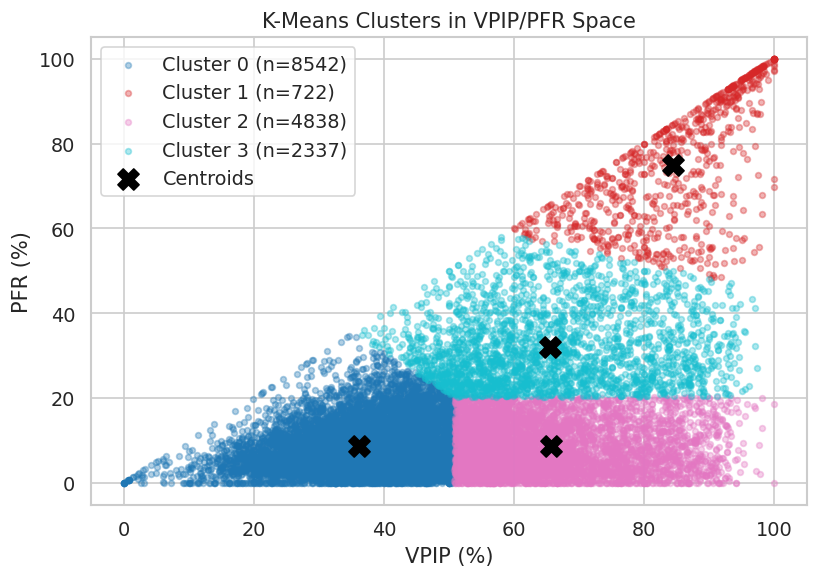
\includegraphics[width=\linewidth]{figures/holdem_kmeans_cluster_scatter.png}
  \caption{K-means clustering results in the VPIP-PFR feature space. Each point represents a player, colored according to cluster assignment. The clustering reveals distinct behavioral groupings corresponding to different levels of looseness and aggression.}
  \Description{Scatter plot of poker players in VPIP-PFR space colored by K-means cluster assignments, showing distinct behavioral player groups.}
  \label{fig:kmeans-clusters}
\end{figure}

\subsection{Comparison Between Heuristics and K-Means}
The heuristic system produced a heavily skewed partition where both Fish and LAG account for 93.5\% of players. On the other hand, Rock and TAG only cover fewer than 7\%. The K-means approach produced a more balanced partition of the player population where cluster sizes ranged from 4.4\% to 52.0\%.

The heuristic LAG category covers a wide region of the feature space and gets split by K-means into three clusters. each cluster has meaningfully different aggression levels. This suggests that the heuristic LAG category contains many behaviorally distinct subgroups. Similarly, heuristic Fish players are distributed across Clusters~0 and~2, suggesting that some players labeled loose-passive actually sit near the tight end of the VPIP spectrum.

K-means merged the heuristic Rock and Tag labels, both of which occupy a small, concentrated region, into Cluster 0. Since these players occupy a small and behaviorally similar region, the K-means approach grouped them together, rather than separating them into distinct categories. 

In summary, K-means discovers structures that fixed, traditional thresholds cannot show, particularly the separation between hyper-aggressive and moderately aggressive players. 

\subsection{Evaluation Metrics}
The quality of the resultant clusters was evaluated using the Silhouette Score. The Silhouette Score, ranging from -1 to +1,  measures how similar each point is to its own cluster relative to the nearest neighboring cluster. Higher values indicate tighter, better separated clusters. 

\begin{table}[t]
  \caption{Silhouette Score Comparison}
  \label{tab:silhouette-comparison}
  \centering
  \begin{tabular}{llr}
    \toprule
    Method & Dataset & Silhouette \\
    \midrule
    Heuristic Baseline & Sampled ($n=344$) & 0.0990 \\
    K-Means ($K=4$) & Sampled ($n=344$) & 0.4595 \\
    \midrule
    Heuristic Baseline & Full ($n=16{,}439$) & 0.1347 \\
    K-Means ($K=4$) & Full ($n=16{,}439$) & 0.4420 \\
    K-Means ($K=2$) & Full ($n=16{,}439$) & 0.4917 \\
    \bottomrule
  \end{tabular}
\end{table}

On the full dataset, K-means at $K=4$ achieves a silhouette score of 0.4420, more than three times the heuristic score of 0.1347. The same pattern is shown in the sampled subset (0.4595 vs.\ 0.0990). This suggests that the result is consistent across both sampled and full datasets. The heuristic's low score is largely due to its LAG category, which covers a wide, heterogeneous region of the feature space.

Model selection across $K=2$ to $K=8$ showed that the highest silhouette score occurs at $K=2$ (0.4917). This indicates that the strongest natural split in the data is binary, most likely separating tight from loose players. Although $K=2$ achieved the highest silhouette score, $K=4$ was selected to match with the number of established poker archetypes. This compromise between cluster quality and ease of interpretation allowed for a direct comparison with the heuristic profiling framework. Figure~\ref{fig:silhouette-plot} shows that a majority of players achieve positive silhouette scores under the $K = 4$ model.  

\begin{figure}[t]
  \centering
  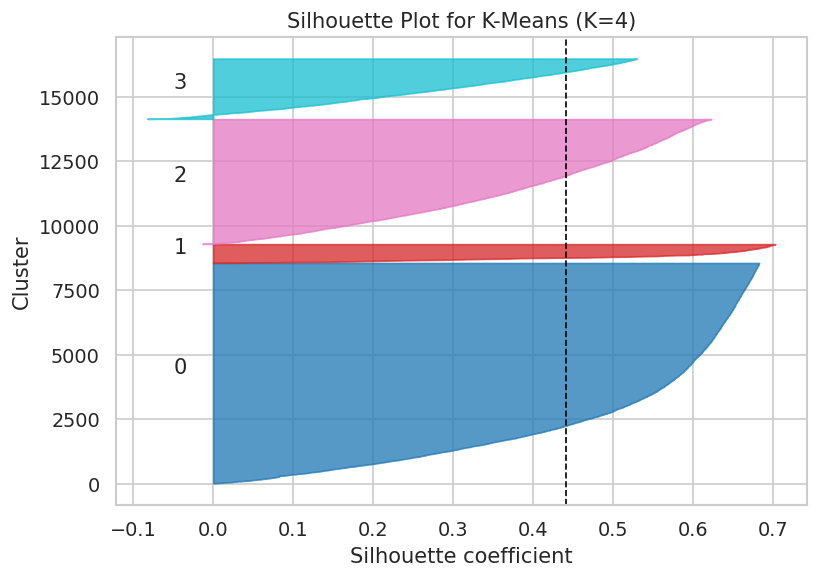
\includegraphics[width=\linewidth]{figures/holdem_kmeans_silhouette_plot.png}
  \caption{Per-sample silhouette plot for the $K=4$ K-means model. Each bar represents one player, grouped by cluster.}
  \Description{Silhouette plot showing per-player silhouette coefficients grouped by cluster assignment.}
  \label{fig:silhouette-plot}
\end{figure}

\section{Conclusion and Future Work}
This section summarizes the main findings of the project, discusses the limitations of the current approach, and outlines potential directions for future research.

\subsection{Conclusion}
This project compared rule-based heuristic profiling with K-means clustering for categorizing poker players using VPIP and PFR features extracted from 16,439 players in the IRC Poker Database.

The main finding is that K-means produces more compact and well-separated groupings than the heuristic baseline under silhouette-based evaluation. At $K=4$, the K-means approach achieves a silhouette score of 0.4420 compared to 0.1347 for the heuristic. This gap is consistent across both the full dataset and a sampled subset. The heuristic's low score is caused primarily by its broad LAG category, which groups players with PFR values ranging from 15\% to 100\% under a single label.

K-means also reveals structure that fixed thresholds did not show. The algorithm separates hyper-aggressive players, such as Cluster~1 with a PFR of~74.9\%, from moderately aggressive ones, such as Cluster~3 with a PFR of~32.0\%. This distinction was invisible under the heuristic system. The strongest natural divide of the data is binary ($K=2$, silhouette 0.4917), suggesting that tight-vs-loose is the most prominent behavioral divide.

However, there are several limitations. In the two approaches, only pre-flop actions were used and post-flop behavior was disregarded. Each player was represented only by a single static average, which does not capture the changes in strategy over time. Secondly, K-means assumes roughly spherical clusters, which may not match the true shape of player behavior distributions.

Despite the limitations, the results show that even a simple unsupervised method, such as K-means, on two features can create better-separated and more compact groupings than the heuristic method under silhouette-based evaluation.

\subsection{Future Work}
As previously discussed, the dataset used in this project consists of poker hand histories collected between 1995 and 2001. Due to the historical nature of the data, the behavioral patterns identified in our analysis may not fully reflect modern poker strategies and gameplay dynamics. Poker strategy has evolved significantly over time as players have adopted more advanced analytical techniques and game-theoretic strategies.

For future work, we would like to extend this analysis by using more recent poker datasets, particularly from the post-2010 era. With access to modern gameplay data, we would be able to conduct a study on how player behavior and strategic tendencies have changed over time, especially across major economic and technological shifts within online poker environments. However, obtaining contemporary large-scale poker datasets is challenging because hand histories are often proprietary and not publicly released due to the competitive nature of the game. Future efforts would therefore involve collaborating with academic researchers or organizations that have access to modern poker gameplay archives.

Future work could also incorporate post-flop actions, winnings, showdown behavior, and temporal changes in player strategy to build more informational player profiles.

\section{Contribution Statement and Peer Evaluation}
\begin{itemize}
    \item \textbf{Lakshya Jain: } Contributed to data pre-processing, feature engineering, K-means clustering analysis, visualization generation, and preparation of the report, presentation, and project website.
    \item \textbf{Aryan Shah: } Contributed to the abstract, analysis, report writing, presentation preparation, and project website development.
    \item \textbf{Shreya Aravindan: } Contributed to analysis, report writing, presentation preparation, and project website development.
    \item \textbf{Claire Shin: } Contributed to exploratory data analysis and pre-processing, and assisted with analysis, the report, presentation, and project website.
\end{itemize}

\bibliographystyle{ACM-Reference-Format}
\bibliography{reference}

\end{document}